% !TEX root = ../main.tex
\section{Training} \label{sec:training}

\subsection{Progressive Pre-Training}
Large-scale video pre-training is highly challenging to optimize when high-resolution videos, multiple conditioning modalities, and heterogeneous data sources are introduced simultaneously from the beginning of training~\cite{ho2022imagen,blattmann2023stable,wan2025wan}. For a sparse Mixture-of-Experts (MoE) diffusion model, this challenge is compounded by the need for the router to establish specialized expert pathways across different tasks and modalities~\cite{shazeer2017moe,switchtransformer,dai2024deepseekmoe}. Exposing the model to full-scale training complexity from the outset may therefore increase the risk of optimization instability, routing collapse, and suboptimal sample quality~\cite{switchtransformer,park2024switch}.

To address these challenges, we design a progressive pre-training curriculum that introduces learning objectives in an optimization-friendly order~\cite{ho2022imagen,blattmann2023stable}. The curriculum first builds stable frame-level visual priors, then adds temporal modeling, expands task conditioning, harmonizes the data distribution, and finally refines high-resolution details. This staged design separates static appearance learning from dynamic evolution and allows the sparse router to specialize gradually rather than being exposed to all sources of heterogeneity at once~\cite{singer2022make,guo2023animatediff}. We organize the curriculum into five stages, each adding one source of training complexity to the previous stage.

\noindent\textbf{Stage 1: Image-Only Prior Acquisition.}
The first stage establishes fundamental text-visual semantic alignment and robust single-frame visual priors~\cite{chen2023pixart,esser2024scaling}. By formulating images as single-frame ($T=1$) video sequences within our unified framework, we enable the model to learn object shapes, textures, and scene aesthetics without the added complexity of temporal dynamics~\cite{singer2022make,guo2023animatediff}. Crucially, this image-first warmup provides a stable optimization environment for the sparse router, allowing it to initialize effectively before encountering heterogeneous video tasks~\cite{switchtransformer,dai2024deepseekmoe}.

\noindent\textbf{Stage 2: Low-Resolution Temporal Learning.}
Stage 2 introduces video data into the image-video training mixture while deliberately maintaining a simplified task formulation. Image samples continue to reinforce frame-level visual priors, while video samples are trained with text-to-video (T2V) generation so that the model can focus on temporal dynamics, camera motion, and frame-to-frame consistency before addressing multi-condition formatting~\cite{ho2022video,bar2024lumiere}. This phase adapts static visual priors into coherent temporal representations without abruptly escalating the optimization difficulty~\cite{singer2022make,guo2023animatediff}.

\noindent\textbf{Stage 3: Multi-Task Conditioning.}
Stage 3 keeps image samples in the training mixture and broadens the video-side task definition from pure T2V to a joint mixture of T2V and text-image-to-video (TI2V) generation~\cite{blattmann2023stable,wan2025wan2}. The primary objective is to teach the model to effectively leverage visual conditions: in the TI2V task, the model must faithfully preserve the provided initial frame while predicting temporally coherent future frames~\cite{esser2023structure,wan2025wan2}. By introducing this requirement only after foundational temporal learning has stabilized, we avoid conflating early motion acquisition with the more challenging constraint of visual condition preservation.

\noindent\textbf{Stage 4: Weighted Distribution Harmonization.} 
Stage 4 focuses on optimizing the data distribution. Large-scale web data exhibits severe quality variance and source imbalance, which can degrade training stability and expert specialization in late-stage pre-training. We therefore switch to a weighted sampler, which samples from high-value and high-quality data sources according to predefined sampling weights via alias tables. This stage lets the model stabilize under a cleaner and more balanced mixture before entering the final refinement phase.

\noindent\textbf{Stage 5: High-Resolution Refinement.}
The final stage functions as a high-resolution refiner, trained on video data. Its primary purpose is to dedicate training capacity to the generation of high-frequency spatial details and the correction of local artifacts in high-resolution samples, all while maintaining temporal sharpness in videos (e.g., minimizing texture flickering)~\cite{saharia2021sr3,ho2022imagen,flashvideo}. Following the cascaded refiner configuration described in~\cref{sec:method}, this stage optimizes a conditional refinement trajectory. It maps upsampled low-resolution base-stage outputs to clean high-resolution targets, ensuring the model retains the base-stage semantics and motion dynamics while successfully restoring fine-grained spatial details~\cite{blattmann2023stable,flashvideo}.


\subsection{Post-Training}
% \todo{jiaqi,chaoran,zijing,zichen}
\subsubsection{Reinforcement Learning with Multi-Aspect Rewards}
\label{sec:training:reward}
\noindent \textbf{Reward Modeling.} 
Existing reinforcement learning (RL) methods in post-training for visual generation typically rely on holistic reward models that output a single scalar score to represent overall human preference or general text-alignment~\cite{xu2023imagereward,kirstain2023pickscore,tang2026enhancing}.
However, video generation is inherently multi-dimensional and prone to complex failure modes, such as static mode collapse, temporal hallucinations, and physical implausibility, which global, coarse-grained rewards fail to penalize effectively.
To address this and provide fine-grained optimization signals, we decouple the evaluation into a comprehensive suite of six specialized reward models to optimize visual quality and physical dynamics during the training process: vision quality, text-video alignment, dynamic degree, motion coherence, human motion consistency, and physical plausibility.
\begin{itemize}
    \item \textbf{Vision Quality.} Following LongCat-Video~\cite{longcatvideo}, we employ HPSv3~\cite{ma2025hpsv3} as the foundation for VQ evaluation to jointly assess visual quality and text-video alignment. We leverage different statistics over all frames in the video to design complementary reward signals that separately capture overall visual fidelity and robust caption alignment. The resulting composite reward penalizes blurriness, artifacts, and low-resolution outputs while remaining sensitive to caption-level alignment.
    
    \item \textbf{Text-Video Alignment.} 
    We propose a fine-grained, action-centric text-video alignment reward based on temporal Visual Question Answering (VQA) to evaluate text-video alignment. 
    We first parse the training caption into structured entities, associating each with specific actions and precise temporal windows. To ensure evaluation accuracy while reducing computational overhead, we introduce an adaptive temporal slicing strategy with a bifurcated windowing mechanism: dynamic actions receive padded windows, whereas static-temporal criteria enforce strict boundaries. We then employ Qwen3.6-27B~\cite{qwen3.6-27b} as a zero-shot evaluator to answer batched verification queries on the sliced frames. 
    The text-video alignment reward is computed as a weighted satisfaction rate normalized to $[0, 1]$, where weights are dynamically assigned based on action complexity. 
    Unlike traditional global semantic matching metrics, this fine-grained approach ensures that accurately generating multi-stage actions yields a significantly higher reward, effectively penalizing temporal hallucinations and missing actions.

    \item \textbf{Dynamic Degree.} 
    We introduce a Dynamic Degree reward evaluated by Qwen3.6-27B~\cite{qwen3.6-27b} to measure and encourage appropriate motion intensity. 
    Specifically, the generated video is spatially downsampled to a maximum height of 480p for efficiency and evaluated using a specialized motion-assessment prompt. 
    The VLM outputs a structured information containing a discrete motion score from 1 to 5, which we linearly map to a continuous reward scalar in $[0, 1]$. 
    By relying on a VLM rather than traditional optical flow, this reward captures semantically meaningful subject dynamics. This counteracts the tendency of text-to-video models to generate static, image-like sequences, effectively breaking the static mode collapse without compromising temporal consistency.

    \item \textbf{Motion Coherence.}
    Text-to-video models generate videos at a fixed playback frame rate (e.g., 24\,fps), yet the generated motion often suffers from a slow-motion effect: it looks slower than it would in the real world, as if captured by a high-speed camera but played back at 24\,fps.
    Following Pulse-of-Motion~\cite{gao2026pulse-of-motion}, we estimate from the generated frames alone how fast the motion actually unfolds.
    The reward mechanism is designed to guide the model toward generating motion that appears natural at a standard 24 fps playback rate. It fully rewards content exhibiting realistic physical speed while penalizing outputs that display an artificial slow-motion effect, thereby steering the model to produce videos with naturally paced dynamics.
    
    \item \textbf{Human-Motion Consistency.} 
    We train a generative human-motion consistency model using a comprehensive distillation approach to evaluate human motion. 
    We build a high-quality dataset of real and synthesized videos to generate five-dimensional artifact scores, specifically targeting impossible topology, facial distortion, hand deformity, limb count errors, and semi-transparent bodies, along with step-by-step reasoning to assess both spatial correctness and temporal fidelity. 
    We subsequently fine-tune a vision-language mixture-of-experts model~\cite{qwen3.6-27b} on this curated corpus. 
    By enforcing supervision over the explicit reasoning traces, the model transcends superficial scalar regression, thereby internalizing the underlying structural and semantic constraints. During the reinforcement learning stage, it outputs structured rationales and discrete scores, which are mapped to a continuous reward scalar in $[0, 1]$. 
    This mechanism explicitly addresses the spatial distortions and temporal-semantic misalignments, guiding the policy toward physically plausible and text-aligned human motion.

    
    \item \textbf{Physical Plausibility.}
    We introduce a Physical Plausibility reward to assess whether generated video trajectories unfold within a coherent physical scene, where task-relevant entities remain present, spatially grounded, and consistent with the intended task evolution. 
    Rather than measuring only perceptual quality, this evaluator is caption-conditioned and frame-evidence-based: it establishes the expected actors, target objects, and final-state cues from the caption, but assigns scores solely based on visible phenomena in the sampled frames.
    It first assesses foundational physical constraints along three complementary axes: motion causality, which verifies whether objects remain stationary or continue moving unless affected by a plausible external force; object permanence and non-penetration, which checks for boundary loss, penetration, impossible overlap, and unsupported appearance or disappearance; and material-kinematic realism, which examines whether entities follow plausible material behavior and rigid-body motion.
    Building upon these physical foundations, the evaluator also incorporates an assessment of task completion. It verifies that the intended physical state changes actually materialize by checking for correct action occurrence, accurate object manipulation, and the successful achievement of the specified final spatial state.
    The resulting scores are aggregated into a unified physical reward. By jointly evaluating adherence to fundamental physical laws and the realization of task-driven state changes, this design ensures that generated videos maintain a coherent, physics-based world where dynamic manipulations and state changes are both visually grounded and physically plausible.
\end{itemize}

\noindent \textbf{Reward Aggregation.}
The six reward signals are aggregated into a single advantage through decoupled per-reward normalization, described in~\cref{sec:training:grpo}.

\subsubsection{On-Policy GRPO Training}
\label{sec:training:grpo}

We post-train {\method} with Group Relative Policy Optimization (GRPO)~\cite{shao2024deepseekmath,liu2025flowgrpo,xue2025dancegrpo} to maximize the multi-aspect rewards. Our setup follows the single-step exploration paradigm of Flash-GRPO~\cite{he2026flashgrpo}: each rollout is stochastic at exactly one denoising step shared within a group, the noise is injected via Coefficients-Preserving Sampling (CPS)~\cite{wang2025cps}, the policy gradient is reweighted to balance timesteps, and training is strictly on-policy without KL regularization. We detail each component below.

\noindent\textbf{Group-Shared Single-Step Exploration.}
GRPO estimates advantages by comparing a group of $G$ rollouts of the same prompt, which requires stochastic sampling. In Flow-GRPO and DanceGRPO~\cite{liu2025flowgrpo,xue2025dancegrpo}, every denoising step is stochastic and all steps share the same trajectory-level advantage, which causes a severe credit-assignment problem~\cite{he2025tempflow,li2025mixgrpo,longcatvideo}. Following Flash-GRPO~\cite{he2026flashgrpo}, we instead make exactly one denoising step stochastic. For each group, a step index $k$ is drawn uniformly from the first half of the inference schedule and shared by all $G$ rollouts. The transition $t_k \to t_{k+1}$ is sampled stochastically, while all other steps remain deterministic ODE steps. Each trajectory then contains exactly one stochastic transition, advantages within a group are compared at the same timestep, and the policy update is applied exactly to the transition that produced the variation, giving precise credit assignment.

\noindent\textbf{Coefficients-Preserving Sampling.}
For the stochastic step we adopt CPS~\cite{wang2025cps}, a DDIM-style transition~\cite{song2020ddim}, instead of the common SDE conversion~\cite{liu2025flowgrpo}. The Euler--Maruyama step of the converted SDE injects more noise than the schedule prescribes~\cite{wang2025cps}, leaving visible artifacts that corrupt reward scores, and its diffusion coefficient explodes at high noise levels, requiring an extra clipping patch~\cite{longcatvideo}; CPS avoids both by construction. Let $1 = t_0 > t_1 > \cdots > t_N = 0$ be the inference schedule. At step $t_i$, the velocity prediction $\hat{v}_\theta$ gives the clean and noise estimates:
\begin{equation}
\hat\x_0 = \x_{t_i} - t_i \hat{v}_\theta, \qquad \hat{\epsilon} = \x_{t_i} + (1 - t_i) \hat{v}_\theta.
\end{equation}
The CPS transition to $t_{i+1}$ is:
\begin{equation}
\x_{t_{i+1}} = \mu_\theta + s_i \epsilon, \qquad
\mu_\theta = (1 - t_{i+1}) \hat\x_0 + \sqrt{t_{i+1}^2 - s_i^2}\, \hat{\epsilon},
\label{eq:cps}
\end{equation}
where $\epsilon \sim \mathcal{N}(0, \mathbf{I})$ is fresh Gaussian noise, $s_i = t_{i+1} \sin(\eta\pi/2)$ is the injected noise scale, and $\eta \in [0, 1]$ controls the exploration strength ($\eta = 0.7$ in our experiments). Since $(t_{i+1}^2 - s_i^2) + s_i^2 = t_{i+1}^2$, the total noise after the transition matches the schedule coefficient exactly: samples stay on the marginal path of the deterministic sampler, and rewards are always evaluated on clean videos. Following~\cite{wang2025cps}, the transition log-likelihood takes the simplified form $\log \pi_\theta(\x_{t_{i+1}} \mid \x_{t_i}) \propto -\lVert \x_{t_{i+1}} - \mu_\theta \rVert^2$.

\noindent\textbf{Timestep-Balanced Gradient Reweighting.}
The strength of the policy gradient at step $k$ scales with the transition gain:
\begin{equation}
\kappa_k = 2 s_k \left| \frac{\partial \mu_\theta}{\partial \hat{v}_\theta} \right|, \qquad
\frac{\partial \mu_\theta}{\partial \hat{v}_\theta} = (1 - t_k)\, t_{k+1} \cos\!\left(\frac{\eta\pi}{2}\right) - t_k (1 - t_{k+1}),
\end{equation}
which varies strongly across the schedule, so a uniformly sampled critical step would let a few timesteps dominate training~\cite{he2026flashgrpo,he2025tempflow,longcatvideo}. We reweight each transition by the inverse gain, normalized to unit mean over the schedule:
\begin{equation}
\lambda_k = \frac{\kappa_k^{-1}}{\frac{1}{N} \sum_{j=0}^{N-1} \kappa_j^{-1}}.
\end{equation}
Here, $N$ is the number of inference steps, and the normalizer is computed analytically over the schedule grid rather than from batch statistics, since all samples in an update batch share one timestep. This equalizes update magnitudes across timesteps without changing the effective learning rate.

\noindent\textbf{Multi-Reward Advantage Normalization.}
The rewards of~\cref{sec:training:reward} have different scales and variances, so we normalize each reward independently before fusing them with weights~\cite{liu2026gdpo}:
\begin{equation}
\hat{A}^{(i)} = \sum_{r} w_r \frac{R_r\big(\x_0^{(i)}, c\big) - \mu_r}{\sigma_r + \delta},
\end{equation}
where $R_r(\x_0^{(i)}, c)$ is the $r$-th reward of sample $i$ under prompt $c$, $w_r$ is its weight, $\mu_r$ and $\sigma_r$ are the mean and standard deviation of $R_r$ within the group, and $\delta$ is a small constant.

\noindent\textbf{Objective.}
The final loss is the reweighted policy gradient on the sampled critical transitions:
\begin{equation}
\mathcal{L}_{\mathrm{GRPO}}(\theta) = - \E\left[ \lambda_k\, \hat{A}^{(i)} \log \pi_\theta\big(\x_{t_{k+1}}^{(i)} \mid \x_{t_k}^{(i)}\big) \right].
\end{equation}
Each rollout batch is consumed by a single gradient update, so training is strictly on-policy and importance ratios stay at one. Following~\cite{xue2025dancegrpo,he2026flashgrpo,xue2026videoposttrain}, we use no KL penalty and no reference model, and we fine-tune all model parameters.

\subsubsection{Negative-Aware Finetuning with Real-World Videos}
\label{sec:training:NFT}

Most existing RL post-training methods for diffusion models rely on reward models to provide optimization signals~\cite{liu2025flowgrpo,xue2025dancegrpo}, which introduces the risk of reward hacking in the video domain. 
To mitigate this, we leverage real-world videos as direct preference signals: a real video clip serves as the positive (chosen) sample, while the model-generated video under the same prompt serves as the negative (rejected) sample. 
This data configuration shares a similar motivation with RealDPO~\cite{guo2025realdpo}, which also pairs real videos with generated ones. 
For the optimization we adopt the forward-process optimization framework of DiffusionNFT~\cite{zheng2026diffusionnft}, bypassing the need to backpropagate through denoising trajectories. 

\noindent\textbf{Preference Pair Construction.}
At each training step, we sample a batch of real video clips from a curated dataset and encode them through the pretrained VAE into clean latents $\x_0^w$ (chosen). 
The active policy generates $N$ videos per prompt via the inference pipeline, and their VAE latents form the rejected pool $\{\x_{0,i}^l\}_{i=1}^N$.
Each rejected latent $\x_0^l$ is paired with the corresponding chosen latent $\x_0^w$ to form a preference pair.
Both latents are perturbed to a shared random timestep $t \sim \mathcal{U}(0, 1)$ with a shared noise vector $\boldsymbol{\varepsilon} \sim \mathcal{N}(\mathbf{0}, \mathbf{I})$:
\begin{equation}
\x_t^w = (1 - t) \x_0^w + t \boldsymbol{\varepsilon},
\qquad
\x_t^l = (1 - t) \x_0^l + t \boldsymbol{\varepsilon}.
\end{equation}
The clean latent is recovered from the noised state via $\hat{\x}_0 = \x_t - t \cdot \hat{v}$, where $\hat{v}$ denotes the predicted velocity.
Operating on single-step noised states avoids trajectory-level log-probability computation, keeping each update computationally lightweight.

\begin{figure}[!ht]
    \centering
    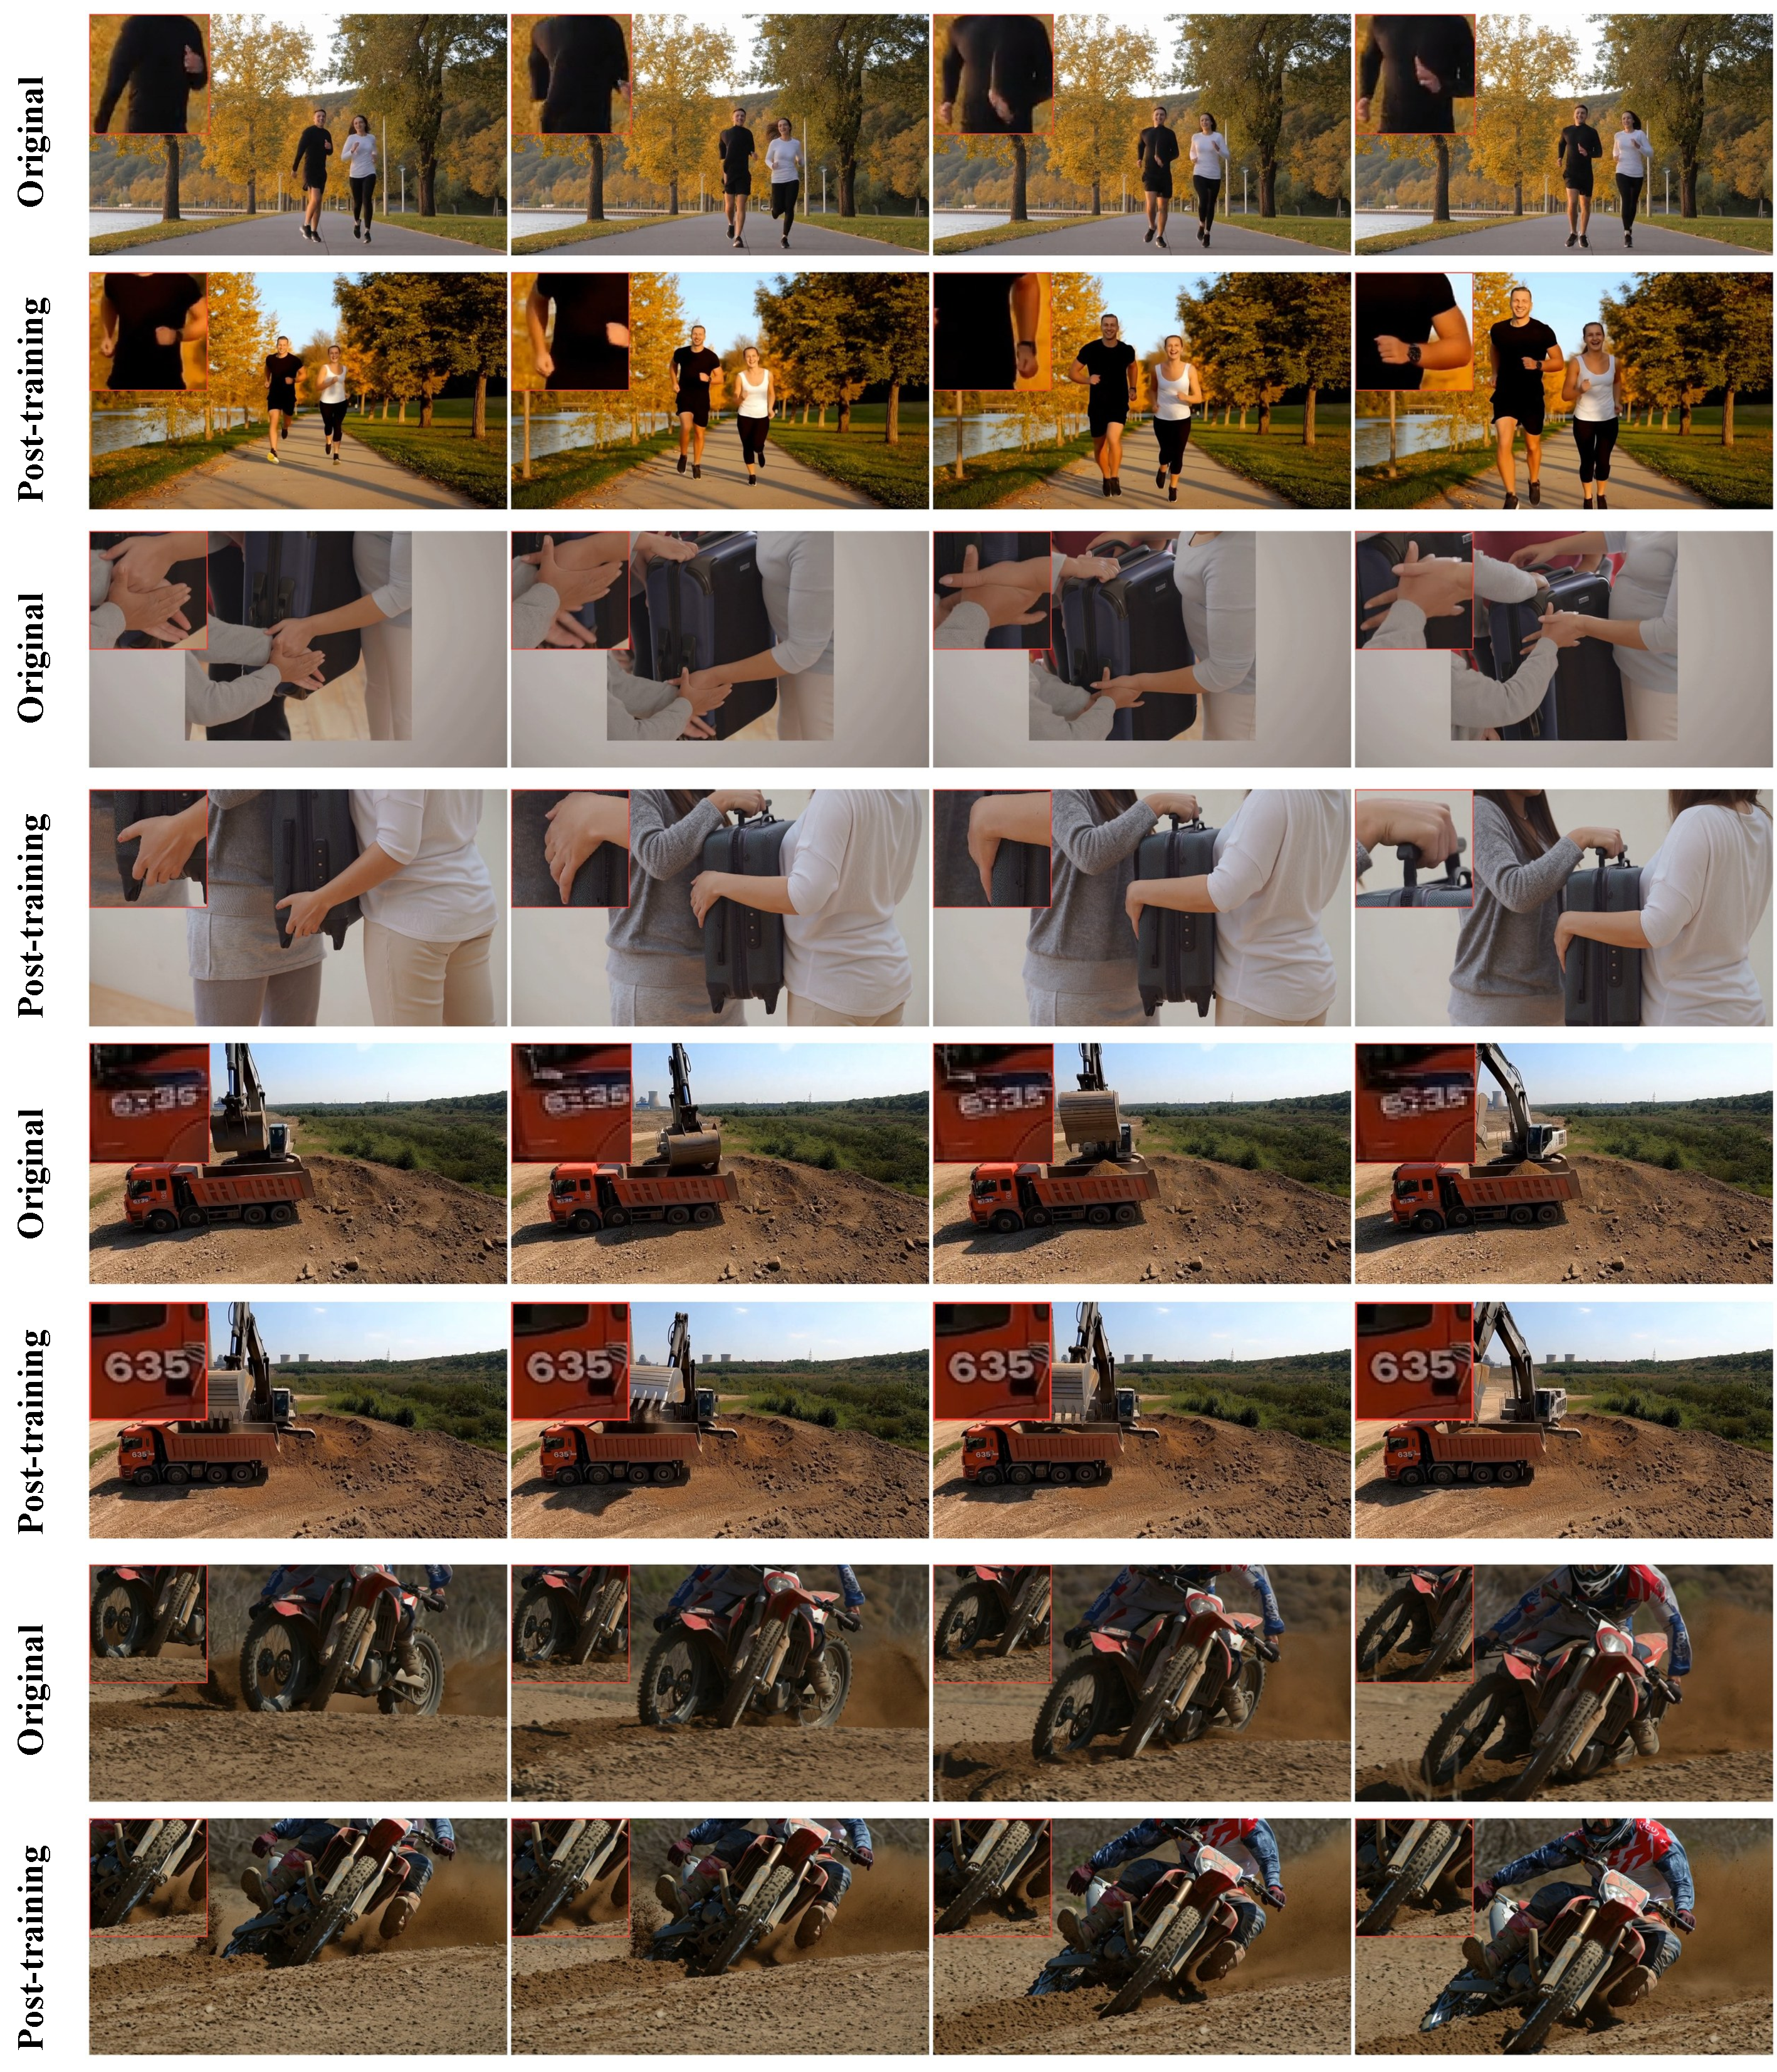
\includegraphics[width=0.95\linewidth]{./figures/rl/rl_improvement_1.pdf}
    \caption{Qualitative comparison on general video quality before and after post-training, demonstrating marked improvements in several fundamental video generation domains. Post-training effectively resolves critical artifacts including inconsistent hand and limb synthesis, blurred or incorrect text rendering, and structural object deformation.}
    \label{fig:rl_general}
\end{figure}

\begin{figure}[!ht]
    \centering
    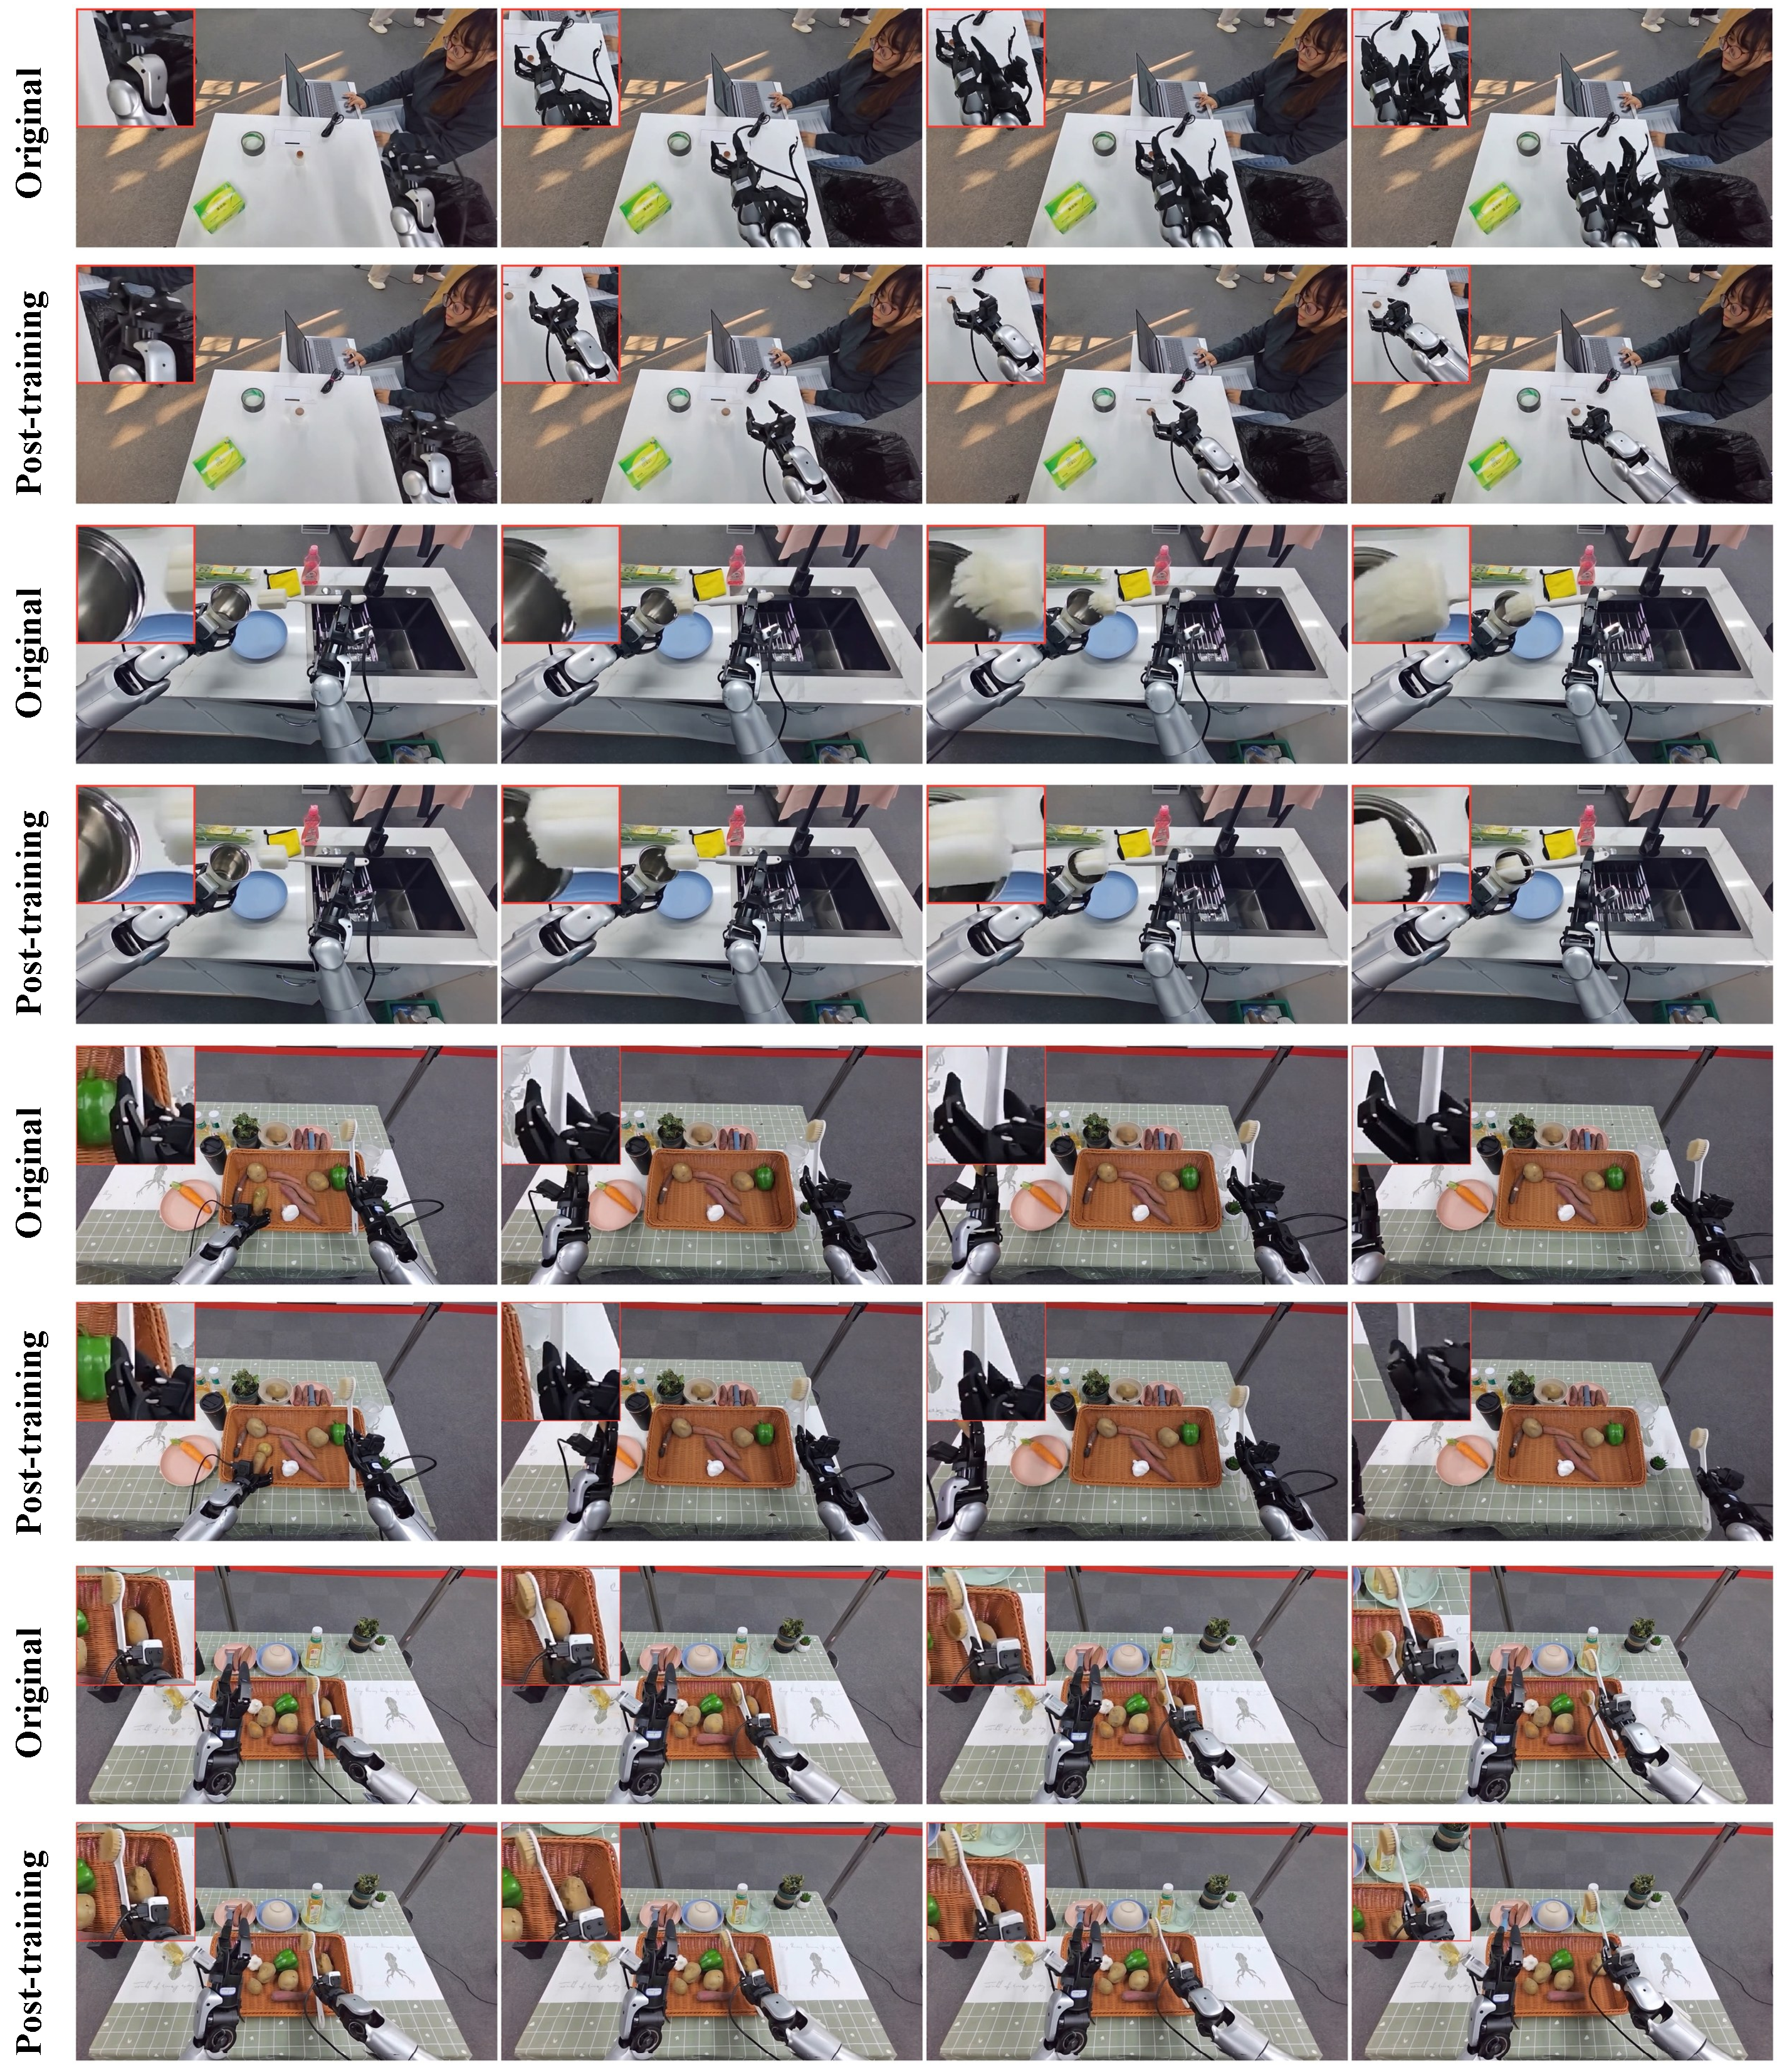
\includegraphics[width=0.95\linewidth]{./figures/rl/rl_improvement_2.pdf}
    \caption{Qualitative comparison on embodied scenarios before and after post-training. The post-training phase significantly enhances physical plausibility by resolving baseline artifacts such as structural distortion of the arm and grasped objects, non-physical penetration, premature object release, and object duplication.}
    \label{fig:rl_embodied}
\end{figure}

\noindent\textbf{Negative-Aware Optimization.}
We maintain two prediction pathways sharing the same base model: (i) the \emph{active policy} $\theta$, which receives gradients; and (ii) the \emph{old policy}, an exponential moving average (EMA) copy of $\theta$ that stabilizes the optimization by preventing the active policy from changing too rapidly.
For any noised state $\x_t^s$ ($s \in \{w, l\}$), the two pathways produce velocity predictions $\hat{v}_{\theta}^s$ and $\hat{v}_{\text{old}}^s$.

Following DiffusionNFT~\cite{zheng2026diffusionnft}, we construct an implicit positive policy that blends the active and old velocity predictions to imitate the target, and an implicit negative policy that extrapolates past the old policy to suppress it:
\begin{align}
\hat{v}_{\text{pos}} = \beta \hat{v}_{\theta} + (1-\beta) \hat{v}_{\text{old}}, \qquad
\hat{v}_{\text{neg}} = (1+\beta) \hat{v}_{\text{old}} - \beta \hat{v}_{\theta},
\end{align}
where $\beta \in (0,1]$ controls how strongly the active policy is allowed to deviate from the old policy.
DiffusionNFT defines the per-sample loss as a reward-weighted mixture of positive and negative branches:
\begin{equation}
\Loss_{\text{NFT}}(r) = r \big\| \hat{v}_{\text{pos}} - v \big\|^2 + (1 - r) \big\| \hat{v}_{\text{neg}} - v \big\|^2,
\end{equation}
where $v = \boldsymbol{\varepsilon} - \x_0$ is the ground-truth flow matching velocity and $r \in [0,1]$ is a normalized reward.

\noindent\textbf{Pairwise Preference Adaptation.}
We adapt this formulation to our pairwise setting by treating the real video as the optimal sample ($r = 1$) and the generated video as the negative sample.
This yields:
\begin{equation}
\Loss_{\text{chosen}} = \Loss_{\text{NFT}}(1)^w = \big\| \hat{v}_{\text{pos}}^w - v^w \big\|^2,
\qquad
\Loss_{\text{reject}} = \Loss_{\text{NFT}}(r)^l = r \big\| \hat{v}_{\text{pos}}^l - v^l \big\|^2 + (1 - r) \big\| \hat{v}_{\text{neg}}^l - v^l \big\|^2.
\end{equation}
In principle, $r$ for the rejected sample could be assigned by a reward model according to generation quality. 
For simplicity and to avoid introducing reward model overhead, we set $r = 0$. 
We also regularize the active policy against a frozen copy of the base model to prevent the policy from drifting too far during fine-tuning:
\begin{equation}
\Loss_{\text{KL}} = \tfrac{1}{2} \bigl( \|\hat{v}_{\theta}^w - \hat{v}_{\text{ref}}^w\|^2 + \|\hat{v}_{\theta}^l - \hat{v}_{\text{ref}}^l\|^2 \bigr).
\end{equation}
The total training objective is:
\begin{equation}
\Loss_{\text{RealNFT}} = \Loss_{\text{chosen}} + \Loss_{\text{reject}} + \lambda_{\text{KL}} \Loss_{\text{KL}}.
\end{equation}




\subsection{Action-to-Video Post-Training}
\label{sec:training:acwm}

\begin{figure}[htbp]
    \centering
    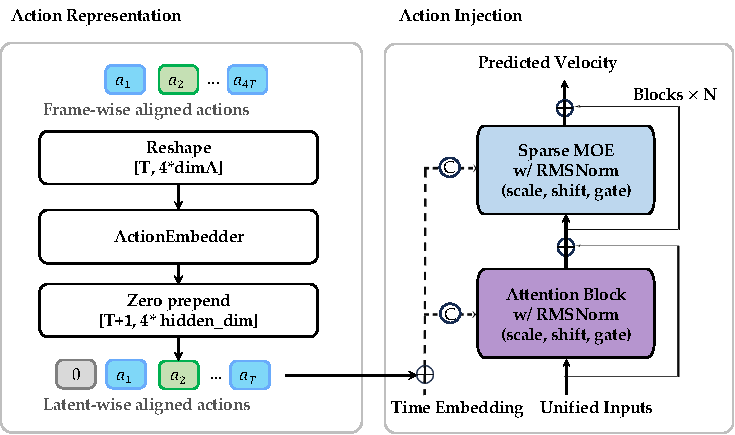
\includegraphics[width=0.7\linewidth]{figures/architecture/acwm.pdf}
    \caption{Architecture of \acwm. Given frame-wise actions for the future $4T$ frames, \acwm first converts the raw commands into relative actions, flattens the action sequence, and maps it with a learnable \texttt{ActionEmbedder} to action latents. A zero action is prepended for the initial state to temporally align action sequence with the $T+1$ visual latents. The action embeddings are injected into the pre-trained transformer blocks with time embeddings.}
    \label{fig:acwm_architecture}
\end{figure}

Embodied world simulation requires a model to roll out plausible future visual trajectories from the current state and a planned action sequence \cite{veorobotics2025,zhu2025unified}.
Beyond visual generation, such simulated futures are central to embodied AI and robot planning, supporting policy evaluation \cite{veorobotics2025,tseng2026sc3}, test-time planning through imagined rollouts \cite{wan2026worldagen}, robot-data scaling via synthetic trajectories \cite{guo2025ctrl}, and reinforcement-learning environments for interactive policy improvement \cite{guo2026vlaw,jiang2026wovr}.
To examine whether \method can transfer its pre-trained understanding of physical rationality, spatial relations, and temporal evolution to this downstream setting, we further post-train it as an action-conditioned world model, denoted \acwm.
Conditioned only on the initial world state, represented by the first image and a textual state description, and on the robot action parameters, \acwm generates action-conditioned visual rollouts of future world states. This setting poses a challenging test of physical-law modeling and action following. We organize the post-training design around three components:
\begin{itemize}
    \item \textit{Data recaptioning.} Pre-trained {\methodname} excels at prompt following, where detailed prompts describe the evolution of the whole video, including physical dynamics and action descriptions. To adapt this simulator into a predictor, we rewrite the data captions so that each prompt describes only the initial state. This encourages the model to drive video evolution using only the given robot actions. We further apply a strict future-leakage check to ensure that the prompts do not reveal future observations or dynamics.
    \item \textit{Action representation and injection.} Given an initial frame and future robot action chunks, we first convert the raw actions into relative actions, so that each step encodes the incremental change from the preceding state. \acwm then flattens the full action chunk into a single sequence and projects it through the \texttt{ActionEmbedder}. As shown in \cref{fig:acwm_architecture}, we prepend a zero action for the initial observation and keep the action latents temporally aligned with the visual latents. The encoded latent-wise aligned actions are injected as residual signals to modulate each transformer block, together with the time embedding. To stabilize post-training, we zero-initialize the last layer of the \texttt{ActionEmbedder}, allowing the newly introduced action branch to be integrated gradually into the pre-trained backbone.
    \item \textit{Training setup.} We adopt the Fourier GR-1 post-training datasets for experiments~\cite{gao2026dreamdojo}. Each training sample follows the same formulation: the model observes the initial world state, receives a sequence of robot actions, and is supervised to generate the corresponding future visual rollout. Starting from the unified pre-trained {\methodname}, we optimize the \texttt{ActionEmbedder} together with the full transformer backbone, rather than training the action branch in isolation, to adapt the original video simulator to predict future frames conditioned on actions. We run post-training for $8k$ steps with a global batch size of 64 and a learning rate of $1e^{-5}$.
\end{itemize}

This adaptation benefits from the synergy between strong pre-trained world priors and targeted action-rollout data. {\methodname} provides action-aware priors over physical-world causality, spatial relations, and temporal evolution, while our recaptioned, leakage-filtered GR-1 trajectories provide clean supervision for action-conditioned rollouts. As a result, \acwm achieves high-quality action following after post-training and can be readily adapted to embodied world simulation. We include additional experimental results in~\cref{sec:eval:acwm}.









\subsection{Distillation}
To improve inference efficiency, we distill \method into a few-step generator following the improved Distribution Matching Distillation (DMD2) framework~\cite{yin2024improved}. Let $G_{\theta}$ denote the student generator conditioned on the unified condition $c$, and let $x_0 = G_{\theta}(z,c)$, where $z \sim \mathcal{N}(0,I)$. For a sampled timestep $t$, we perturb the generated latent video as $x_t = \alpha_t x_0 + \sigma_t \epsilon$. The method matches the student distribution to the teacher distribution by minimizing a reverse-KL-style distribution-matching objective over diffusion noise levels:
\begin{equation}
\nabla_{\theta}\mathcal{L}_{\mathrm{DMD}}
=
\mathbb{E}_{z,t,\epsilon}
\left[
-w_t
\left(
s_{\mathrm{real}}(x_t,t,c)-s_{\mathrm{fake}}(x_t,t,c)
\right)
\frac{\partial G_{\theta}(z,c)}{\partial \theta}
\right],
\end{equation}
where $s_{\mathrm{real}}$ is provided by the teacher video diffusion model, and $s_{\mathrm{fake}}$ is estimated by an auxiliary score model trained online on samples from the current student. We also retain a lightweight GAN objective to provide real-data supervision and improve visual quality.